\documentclass[journal=jctcce,manuscript=suppinfo,layout=traditional]{achemso}
\usepackage[T1]{fontenc}
\usepackage{amsmath,amssymb,booktabs,graphicx,bm}
\newcommand{\vect}[1]{\bm{#1}}
\newcommand{\FACE}{\textsc{face}}
\renewcommand{\thetable}{S\arabic{table}}
\renewcommand{\thefigure}{S\arabic{figure}}
% Author details, shared by main.tex, si.tex and cover_letter.tex. Edit only this file.
\newcommand{\AuthorName}{Albert Linda}
\newcommand{\AuthorAffiliation}{Department of Materials Science and Engineering, Indian Institute of Technology Kanpur, Kalyanpur, Kanpur 208016, Uttar Pradesh, India}
\newcommand{\AuthorORCID}{0000-0002-3723-1756}
\newcommand{\AuthorEmail}{albert.hzbn@gmail.com}
\newcommand{\Funding}{This research received no specific grant from any funding agency in the public, commercial or not-for-profit sectors.}
\newcommand{\AuthorAddressLines}{Department of Materials Science and Engineering\\Indian Institute of Technology Kanpur\\Kalyanpur, Kanpur 208016, Uttar Pradesh, India}

\author{\AuthorName}
\affiliation{\AuthorAffiliation}
\email{albert.hzbn@gmail.com}
\title{Factorised Cartesian Atomic Cluster Expansion for Low-Cost Machine-Learning Interatomic Potentials}

\begin{document}

\section*{S1. Architecture development history (aspirin, rMD17 split 1, 60 epochs)}
Development proceeded by hypothesis-driven changes, each tested on the identical split and budget. Versions v0--v4
predate the unit parameterisation (lr 0.005--0.01); single 60-epoch runs vary by 20--30\% between seeds
(Table~\ref{tab:seeds}), so differences below that level are within noise.

\begin{table}[h]
\caption{Architecture iterations. $E$ (meV) / $F$ (meV/\AA) test MAE. MACE-small control: 10.6 / 19.5.}
\label{tab:history}
\small\setlength{\tabcolsep}{3pt}
\begin{tabular}{lp{5.6cm}p{2.9cm}p{3.2cm}}
\toprule
version & change (hypothesis) & $E$ / $F$ & outcome \\
\midrule
v0 & Cartesian moments, scalar messages & 16.4 / 30.5 & baseline \\
v1 & + bond-projected directional invariants, element-pair radial & 14.1 / 27.3 & better \\
v1 & layer norm $\to$ affine (magnitude information) & 17.9 / 33.7 & rejected \\
v2 & + rank-preserving tensor transport ($C=96$) & 9.2 / 21.2 & better \\
v3 & + gated equivariant products ($C=96$) & 6.8 / 16.7 & best accuracy; edge cost $\propto C$ \\
v4 & factorised edges, $B=16$, $K=32$ & 10.2 / 20.5 & 1.7$\times$ MACE-small speed \\
v4 & wider node layer $C=128$ & 11.0 / 22.0 & no gain: bottleneck is edge rank \\
v4 & $K=64$ / $B=32$ / $K_d=48$ & 10.5/22.6, 8.8/18.1, 8.6/18.0 & radial basis and transport width matter \\
v4 & single pass (strictly local) & 20.3 / 42.5 & rejected \\
v5 & per-atom equivariant RMS normalisation & 20.7 / 32.7 & stable but less accurate \\
v7 & unit parameterisation, lr 0.01 / 0.02 / 0.04 & 12.5/24.1, 9.4/19.4, 8.9/17.6 & adopted (lr 0.04) \\
v7 & flagship $B=16$, $r_c=4.5$~\AA & 8.45 / 18.3 & adopted \\
v7 & $C=64$, $r_c=4.5$~\AA & 11.6 / 21.5 & fastest; less accurate on aspirin \\
v8 & CP edge densities (\FACE-CP) & 7.2 / 16.4 & accuracy option \\
\bottomrule
\end{tabular}
\end{table}

\section*{S2. Training-stability probe}
Constant learning rate, Adam (AMSGrad), batch 5; first optimiser step with a non-finite loss or gradient.

\begin{table}[h]
\caption{Stability probe. ``none'' = no non-finite step within the probe length.}
\label{tab:probe}
\small
\begin{tabular}{lp{6.2cm}p{4.3cm}}
\toprule
molecule, lr, steps & configuration & first non-finite step \\
\midrule
aspirin, 0.01, 400 & calibrated fixed scales, no layer norm & 2 \\
 & same, max body order 3 / 4 & 4 / 2 \\
 & same, no transport and no gated products & 3 \\
 & same, one pass / one pass with body order $\le3$ & 17 / none (no learning) \\
 & same + unit parameterisation & 33 \\
 & layer norm (v4) & none (F-RMSE 315 meV/\AA{} at step 400) \\
 & layer norm + unit parameterisation & none (276) \\
ethanol, 0.01, 1500 & layer norm (v4) & 85 \\
 & layer norm + unit parameterisation & none (F-RMSE 283 $\to$ 107) \\
 & layer norm + unit + calibrated scales & 24 \\
\bottomrule
\end{tabular}
\end{table}
Additional observations: (i) at initialisation, 4- and 5-body invariants are $10^{-6}$--$10^{-9}$ of the 2-body ones,
so they are invisible after layer normalisation; (ii) the optimiser can exploit the scale invariance of layer
normalisation by inflating moment magnitudes, which reweights body orders and eventually overflows the
second-derivative computation; (iii) fixed equivariant saturation ($s=4$) removed all non-finite steps on Ag$_3$ but
doubled the aspirin error (19.5/40.0); (iv) weight decay $10^{-3}$ worsened ethanol accuracy (4.56/17.1 vs
3.08/13.9 for the same seed); (v) the EMA copy of the model must also receive buffers, otherwise calibrated scales are
lost at evaluation.

\section*{S3. Kernel engineering (exact, output-identical changes)}
\begin{table}[h]
\caption{Effect of implementation changes on the flagship (speed ratio to MACE-small, interleaved timing).}
\label{tab:kernels}
\begin{tabular}{lc}
\toprule
change & speed vs MACE-small \\
\midrule
v4 PyTorch baseline & 1.85$\times$ \\
+ fused density kernel (forward 2.1$\times$, backward 150 $\to$ 40 ms) & 2.5--2.7$\times$ \\
+ fused node algebra (6.3$\times$ on the node layer) & 3.2$\times$ \\
+ constant-map transport & 3.65$\times$ \\
+ $r_c$ 4.5~\AA{} (27\% fewer edges) & 4.1$\times$ \\
+ node kernel on symmetric storage & 4.8$\times$ \\
idle-GPU measurement, 1,344 atoms & 5.7$\times$ \\
\bottomrule
\end{tabular}
\end{table}
For \FACE-CP, replacing per-rank slicing of the $(N,M,4,C)$ edge tensor by a single GEMM against all 20 monomials
raised the speed ratio from 2.0$\times$ to 2.9$\times$.

\section*{S4. Ensembles, seed variance and additional distillation results}
\begin{table}[h]
\caption{Seed variance and ensembles (aspirin unless stated; $E$ meV / $F$ meV/\AA).}
\label{tab:seeds}
\begin{tabular}{lc}
\toprule
set & result \\
\midrule
flagship, 400 epochs, 5 seeds & 2.97--3.42 / 8.82--9.60 \\
ethanol flagship, 60 epochs, 3 seeds & 2.87--3.93 / 13.3--16.3 \\
ethanol MACE-small, 60 epochs, 3 seeds & 3.02--3.38 / 13.0--14.5 \\
3 / 5 flagship ensemble & 2.73 / 7.35;\ 2.73 / 7.09 \\
7 / 11 flagship-class ensemble & 2.64 / 6.84;\ 2.50 / 6.67 \\
11-model teacher incl.\ distilled students & 2.55 / 6.53 \\
ethanol, 3 / 4 member ensemble & 0.61 / 3.86;\ 0.60 / 3.73 \\
\bottomrule
\end{tabular}
\end{table}

\begin{table}[h]
\caption{Distillation variants that did not help (aspirin, single models).}
\label{tab:distillneg}
\begin{tabular}{lc}
\toprule
variant & $E$ / $F$ \\
\midrule
flagship student, 1 teacher batch (19k) & 3.49 / 8.32 \\
flagship student, 2 batches (38k), same steps & 3.55 / 8.55 \\
CP student, 1 batch & 3.07 / 7.83 \\
CP student, 3 batches incl.\ 600~K (56k), same steps & 3.37 / 8.32 \\
rank-3 transport student & 3.62 / 8.46 \\
polynomial (linear per-pass) readout, 400 epochs & 3.59 / 9.75 \\
rank-3 transport, 400 epochs, seeds 0/1 & 2.91/8.30, 3.24/9.17 \\
per-element product gates, 400 epochs & 2.97 / 8.82 (within seed spread) \\
\bottomrule
\end{tabular}
\end{table}

\section*{S5. Error metrics, scaling and published reference values}
Table~\ref{tab:rmse} complements the MAE values of the main text with root-mean-square errors on the same 1000 test
structures. RMSE/MAE ratios of 1.4--1.6 (energy) and 1.5--1.9 (force) are similar for \FACE{} and MACE, so the
ranking does not depend on the metric.

\begin{table}[h]
\caption{Energy (meV) and force (meV/\AA) MAE and RMSE, rMD17 test set (1000 structures).}
\label{tab:rmse}
\begin{tabular}{lcccc}
\toprule
model & $E$ MAE & $E$ RMSE & $F$ MAE & $F$ RMSE \\
\midrule
\multicolumn{5}{l}{\emph{aspirin}} \\
flagship, 400 epochs & 3.13 & 4.42 & 9.08 & 13.86 \\
\FACE-CP $C=96$, 400 epochs & 2.88 & 4.59 & 8.73 & 13.61 \\
flagship, distilled & 3.13 & 4.37 & 8.04 & 12.29 \\
\FACE-CP $C=96$, generation 3 & 2.50 & 3.60 & 6.97 & 10.69 \\
\FACE-CP $C=160$, generation 4 & 2.26 & 3.23 & 6.74 & 10.43 \\
MACE-small, 60 epochs & 10.60 & 15.13 & 19.51 & 28.52 \\
MACE-medium, 60 epochs & 9.13 & 12.85 & 17.80 & 26.33 \\
\midrule
\multicolumn{5}{l}{\emph{ethanol}} \\
\FACE-CP, 400 epochs & 0.78 & 1.21 & 4.84 & 8.52 \\
\FACE-CP, distilled (generation 1) & 0.68 & 1.06 & 4.22 & 7.92 \\
\FACE-CP $C=160$, generation 2 & 0.62 & 1.09 & 3.72 & 7.33 \\
MACE-small, 400 epochs & 1.11 & 1.73 & 6.76 & 12.02 \\
\bottomrule
\end{tabular}
\end{table}

\begin{table}[h]
\caption{Inference speed relative to MACE-small versus system size (energy + forces, float32, interleaved timing
rounds, median; periodic boxes of $n^3$ randomly oriented aspirin molecules on a cubic grid, $n=2$--5).}
\label{tab:scaling}
\begin{tabular}{lcccc}
\toprule
atoms & 168 & 567 & 1,344 & 2,625 \\
\midrule
\FACE{} flagship & 2.34$\times$ & 4.67$\times$ & 5.64$\times$ & 5.43$\times$ \\
\FACE-CP $C=96$ & 2.37$\times$ & 2.77$\times$ & 3.20$\times$ & 2.91$\times$ \\
\bottomrule
\end{tabular}
\end{table}

\begin{table}[h]
\caption{Training-step cost: forward pass, forces with \texttt{create\_graph}, $E$/$F$ loss, backward pass and
AMSGrad step on five aspirin molecules (median of seven interleaved rounds of ten steps). Parameter counts are those
of the benchmark construction.}
\label{tab:trainstep}
\begin{tabular}{lccc}
\toprule
model & parameters & step (ms) & relative to MACE-small \\
\midrule
MACE-small & 204,432 & 97.2 & 1.00 \\
MACE-medium & 604,432 & 130.9 & 1.35 \\
\FACE{} flagship & 1.56\,M & 93.4 & 0.96 \\
\FACE-CP $C=96$ & 1.31\,M & 92.6 & 0.95 \\
\FACE-CP $C=160$ & 3.36\,M & 95.1 & 0.98 \\
\bottomrule
\end{tabular}
\end{table}

\begin{table}[h]
\caption{Published rMD17 MAE values ($E$ meV / $F$ meV/\AA, 950 training structures, converged training) for
context; the 60-epoch results of the main text are not converged and are not directly comparable.}
\label{tab:published}
\begin{tabular}{lcccc}
\toprule
model & malonaldehyde & uracil & toluene & ethanol \\
\midrule
NequIP & 0.8 / 5.1 & 0.4 / 3.1 & 0.3 / 1.6 & 0.4 / 2.8 \\
Allegro & 0.6 / 3.6 & 0.6 / 1.8 & 0.4 / 1.8 & 0.4 / 2.1 \\
MACE & 0.8 / 4.1 & 0.5 / 2.1 & 0.5 / 1.5 & 0.4 / 2.1 \\
\bottomrule
\end{tabular}
\end{table}

\begin{table}[h]
\caption{Cost of the physics operators relative to the local flagship (fused kernels and spline radial functions),
energy and forces, periodic aspirin boxes; interleaved timing rounds, medians. Electrostatics: latent charges in
coulomb mode with smooth particle-mesh Ewald; dispersion with a 10~\AA{} pair list.}
\label{tab:operators}
\begin{tabular}{lcccc}
\toprule
atoms & electrostatics & dispersion & ZBL & all three \\
\midrule
567 & +62\% & +12\% & +8\% & +81\% \\
1,344 & +32\% & +9\% & +5\% & +44\% \\
2,625 & +17\% & +10\% & +3\% & +28\% \\
4,536 & +12\% & +12\% & +2\% & +23\% \\
\bottomrule
\end{tabular}
\end{table}

\begin{table}[h]
\caption{Inference time versus model width at 1,344 atoms, relative to MACE with 64 channels measured in the same
interleaved rounds (energy and forces, float32).}
\label{tab:width}
\begin{tabular}{lc}
\toprule
model & time relative to MACE, 64 channels \\
\midrule
MACE, 32 channels & 0.577 \\
MACE, 64 channels & 1.000 \\
MACE, 128 channels & 1.874 \\
\FACE{} $C=32$ & 0.163 \\
\FACE{} $C=64$ & 0.168 \\
\FACE{} $C=96$ & 0.181 \\
\FACE{} $C=128$ & 0.195 \\
\FACE{} $C=192$ & 0.229 \\
\FACE{} $C=256$ & 0.271 \\
\FACE-CP $C=64$ & 0.265 \\
\FACE-CP $C=96$ & 0.342 \\
\FACE-CP $C=160$ & 0.503 \\
\bottomrule
\end{tabular}
\end{table}

\begin{table}[h]
\caption{Peak GPU memory (GB) for one energy and force evaluation, periodic aspirin boxes, float32. OOM: exceeds
the 12~GB cap.}
\label{tab:memory}
\begin{tabular}{lcccc}
\toprule
atoms & \FACE{} flagship & \FACE-CP $C=96$ & MACE, 64 ch. & MACE, 128 ch. \\
\midrule
168 & 0.10 & 0.21 & 0.36 & 0.66 \\
567 & 0.31 & 0.71 & 1.13 & 2.17 \\
1,344 & 0.70 & 1.69 & 2.67 & 5.12 \\
2,625 & 1.39 & 3.38 & 5.20 & 9.97 \\
4,536 & 2.30 & 5.66 & 8.98 & OOM \\
\bottomrule
\end{tabular}
\end{table}

\begin{table}[h]
\caption{Learning curve of the \FACE{} flagship on rMD17 aspirin: nested training subsets, the same 50 validation and
1000 test structures; energy (meV) and force (meV/\AA) MAE.}
\label{tab:learningcurve}
\begin{tabular}{rrccl}
\toprule
$N$ & epochs & $E$ & $F$ & note \\
\midrule
50 & 2000 & 24.60 & 50.30 &  \\
100 & 1000 & 10.74 & 32.20 &  \\
250 & 400 & 7.13 & 19.74 &  \\
500 & 400 & 4.18 & 12.77 & stopped at epoch 380 \\
950 & 400 & 3.13 & 9.08 &  \\
\bottomrule
\end{tabular}
\end{table}

\clearpage
\section*{S6. Hyperparameters}
Two message-passing steps; eight Bessel functions with polynomial envelope ($p=6$); radial MLP width 64 with
element-pair embedding; $K_d=16$ directional and transport channels; nine invariant families with layer
normalisation and an MLP of widths $(9C+C+4)\to2C\to2C\to C+1$; SiLU activations; unit parameterisation of all
linear layers. Optimiser: AMSGrad/AdamW, weight decay 0, peak learning rate 0.04 (one-cycle, 5\% warm-up, initial
and final divisors 10 and 100), batch 5, gradient clipping 10, EMA 0.99, energy-weighted final 25\% of epochs.
Distillation: 25 epochs over DFT$\times4$ plus teacher data; DFT-only fine-tune 60 epochs at $4\times10^{-3}$ (half
energy-weighted); energy-weighted fine-tune 60 epochs at $2\times10^{-3}$ with $(w_E,w_F)=(1000,10)$. Latent charges:
Gaussian width 0.5~\AA, Ewald splitting $\gamma'=r_c/3.5$, SPME grid spacing $\gamma'/4$, order-4 B-splines.

\section*{S7. Entries of the transport map}
With the pooled sums $S_{(p,y)}=\bar n^{-1}\sum_jY_p(\hat{\vect u}_{ij})\phi_b(r_{ij})T_{j,y}$ defined in the
section on tensor transport of the main text (indices $b$ and $k$ omitted), $p\in\{0,1,2,3\}$ for the monomials $\{1,u_1,u_2,u_3\}$ and $y$ running over
the components $V_a$ and $M_{ab}$ ($a\le b$) of the neighbour tensor, the 18 outputs of the $(36\times18)$ map are
\begin{align*}
\textstyle\sum_j\phi_b\,V_{j,a}&=S_{(0,V_a)}, &
\textstyle\sum_j\phi_b\,(\vect M_j\hat{\vect u})_a&=\textstyle\sum_{c=1}^3S_{(c,M_{ac})},\\
\textstyle\sum_j\phi_b\,M_{j,ab}&=S_{(0,M_{ab})}, &
\textstyle\sum_j\phi_b\,\mathrm{sym}(\hat{\vect u}\otimes\vect V_j)_{ab}&=\tfrac12\big(S_{(a,V_b)}+S_{(b,V_a)}\big),
\end{align*}
for $a,b=1,2,3$, with $M_{ac}=M_{ca}$ read from symmetric storage. All other entries are zero, and every non-zero
entry is $1$ or $\tfrac12$. The rank-3 option extends $p$ to the ten monomials of degree $\le2$ and adds the outputs
$\mathrm{sym}(\hat{\vect u}\otimes\vect M_j)$ and $\mathrm{sym}(\hat{\vect u}\otimes\hat{\vect u}\otimes\vect V_j)$,
which are symmetrised sums of the same kind ($(90\times38)$ map). The maps are generated programmatically and tested
against explicit per-edge evaluation.

\section*{S8. Learning curves}
\begin{figure}[h]
\centering
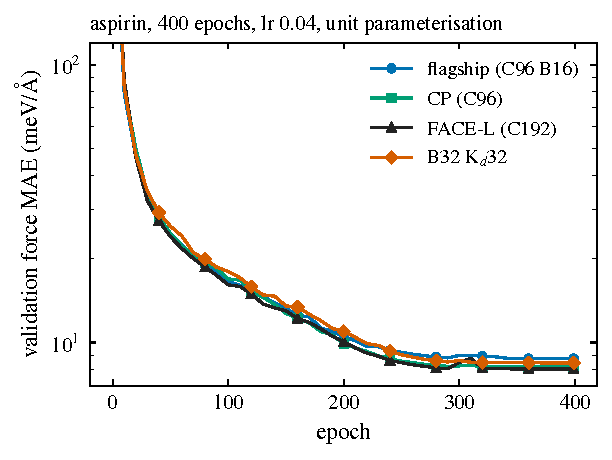
\includegraphics[width=0.6\linewidth]{figures/fig_learning_curves.pdf}
\caption{Validation force MAE during 400-epoch training of four configurations (aspirin).}
\label{fig:lc}
\end{figure}

\end{document}
